\chapter {绪论}
\label{chp:intro}

\section{研究背景}

随着移动市场于近年逐渐兴起,Android系统作为一个主流的移动端操作系统也在蓬勃发展。
数据分析机构StatCounter资料显示,Android市场占有率自发布之日起就在逐年稳步增长。
截至2020年,Android系统已经占据全球移动端市场份额的74.3\%~\cite{MobileOSMktShare}。
与此同时,Android应用的数量也伴随着Android市场的蓬勃发展节节攀高。\footnote{应用、App在本文中均用以指代Android应用程序,下文不再区分}
仅Android官方的应用商店Google Play就在2017年中新上架了近一百万个可供下载的应用程序。
虽然因为各种原因,Google Play上的应用数量在2018年有所回落,但如\autoref{fig:app_number}所示,应用市场上目前仍有近三百万个可用的应用程序,Android应用市场依然充满活力~\cite{StatistaAppNumber}。

\begin{figure}[htbp]
	\centering
	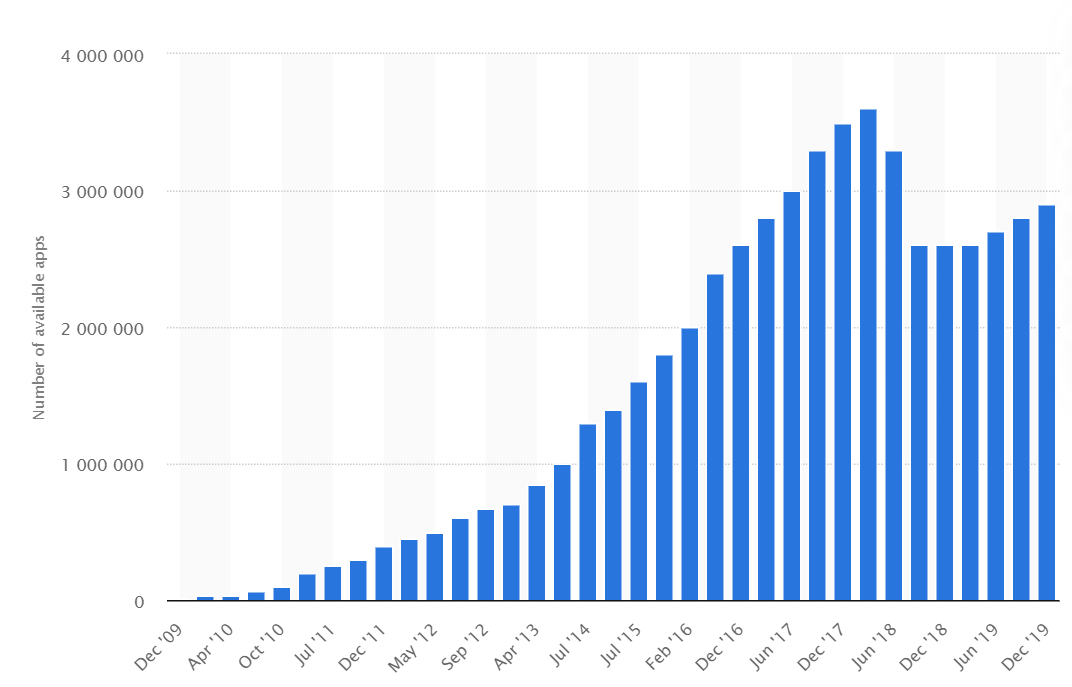
\includegraphics[width=0.9\textwidth]{./Figures/edwin-intro-app-number.png}
	\caption{Google Play 应用商店架上应用总数变化趋势}
	\label{fig:app_number}
\end{figure}

随着Android移动应用行业快速发展,移动黑灰产(即移动端黑色产业与灰色产业,下文同)也逐渐活跃。
黑灰产是以侵害用户、原应用作者或其他第三方利益为手段,凭此或通过其他可疑方式牟利的产业。
一方面,随着开发移动应用的门槛逐渐下降,开发一个移动应用的成本已经普遍低于开发一个类似的桌面级应用所需的成本~\cite{wasserman2010software};
另一方面,移动应用功能在实现上的灵活性~\cite{storydroid}增加了移动应用的复杂度,针对黑灰产的分析与拦截面临着多重新挑战。
两方面结合,为黑灰色应用进入移动端发展提供了良好的基础。

仿冒应用就是一类广泛存在的移动灰黑产产物。
本文研究的仿冒应用指代开发者根据市面上热门应用的外观仿制的Android应用。
据日常观察,仿冒应用中常有恶意广告弹窗、信息窃取、恶意扣费等行为,开发者可在用户使用仿冒应用时利用广告流量或非法获得的用户信息获利。
一方面,仿冒应用损害了原版应用开发者的知识产权,侵害了原开发者的利益;
另一方面,仿冒应用中的恶意行为也在威胁普通用户的信息安全。
可以联想如下场景:用户尝试通过应用市场搜索安装一个应用,应用市场返回了多个无论是名字或是图标都十分相像的结果,在未有明确指引的情况下,用户安装了仿冒应用。
前人针对Android恶意应用的研究~\cite{Zhou2012DissectingAM}显示,恶意行为可被自动触发,若用户下载的仿冒应用中包含此类恶意行为,用户数据安全将受到损害;
同时,由于用户不能分辨原版应用与仿冒应用,后者的不良用户体验会导致用户对前者乃至应用市场产生不良评价;
即使用户删除仿冒应用、装上原版应用,也浪费了时间和人力成本。

综上所述,仿冒应用影响用户搜索与下载应用时的安全和体验,最终使用户、原版应用开发者和应用市场三方利益均受到损害。
为了消除仿冒应用带来的隐患,无论是开发者、应用市场或是普通用户,都有必要对仿冒应用的特征与行为有更深入的理解。

\section{研究现状}
尽管客观上存在对仿冒应用进行了解的需求,本研究对移动应用领域的前期调研显示,针对仿冒应用进行的实证研究尚缺乏,也未有公开可用的仿冒应用数据集。
因此,本节讨论与仿冒应用同属于移动灰黑产的重打包应用和恶意应用、以及其他移动应用领域相关方向的研究现状。

\subsection{重打包应用的研究现状}
\label{sec:study_repackaging}
重打包指恶意开发者对原应用解包、篡改内容之后再将应用重新打包的技术~\cite{khanmohammadi2019empirical}。
重打包应用侵害了应用原作者的知识产权,甚至可能具有恶意行为,因此也属于移动黑灰产范畴。
目前针对重打包应用的相关工作分为三类,分别为关于重打包的实证研究、针对重打包应用的检测和防止应用被重打包的研究。

相关实证研究方面,Khanmohammadi等人对重打包应用进行了一次详尽的实证研究~\cite{khanmohammadi2019empirical}。
该实证研究利用已有数据集AndroZoo~\cite{li2017androzoo++},得出了``重打包应用的主要目的为利用广告获得收入''的结论,并回答了包括``何种类型的应用会被重打包''、``重打包对原应用属性更改如何''在内的五个研究问题,增进了研究者对重打包应用的理解。


在重打包应用检测方面,早期工作通过比对两两应用之间的信息获得应用之间的相似度。
有研究者基于应用指令序列的方法使用模糊哈希的方法提取出应用的摘要信息,如DroidMOSS和DroidAnalytics~\cite{DroidMOSS, Zheng2013DroidAnalyticsA};
也有使用静态数据依赖构建程序依赖图(Program Dependency Graph, PDG)比对应用的方法,如DNADroid~\cite{DNADroid}和AnDarwin~\cite{AnDarwin},Centroid~\cite{Centroid}甚至为应用中的每个函数构建了三维控制流图(3-Dimensional Control Flow Graph, 3D-CFG),将三维控制流图聚合后,通过检测不同应用在控制图聚合后的质心位置判断应用间的相似程度;
还有算法通过比对抽象语义树检测重打包应用,如Hanna等人的Juxtapp~\cite{hanna2012juxtapp}利用K-gram模型对应用的二进制操作码序列进行比对,CLANdroid~\cite{CLANdroid}通过分析五种语义特征点(比如代码中的标识符和调用到的Android API等),以检测相似应用。
上述算法一来因为需要使用静态分析方法对代码进行解析,在遇到使用过代码混淆处理(如反射和代码加密)的应用时性能往往较差;二来需要基于两两比对进行检测,复杂度较高,在应用规模增大时会导致庞大的计算量。
为处理静态分析带来的问题,有学者提出了利用动态分析比对应用的方法,如Wu等人使用HTTP流量对应用行为进行建模~\cite{wu2015detect}。
亦有研究使用信息可视化方法检测重打包应用:ViewDroid~\cite{ViewDroid}通过重建和比对应用的视图筛出重打包应用,DroidEagle~\cite{sun2015droideagle}则利用UI布局相似性检测,Kywe等人比对应用中的文本与图像相似性以寻找相似应用~\cite{kywe2014detecting},Soh等人分析应用运行时收集的UI信息以检测重打包行为~\cite{soh2015detecting}。
而从避免两两比对、减小算法复杂度方面考虑,有学者提出利用第三方库进行检测的办法,如CodeMatch~\cite{CodeMatch}筛选出应用中使用的第三方库代码后,计算并比对剩余部分代码的哈希值,获取不同应用的相似程度;Wukong~\cite{Wukong}也分两步检测重打包应用,但与CodeMatch相比,其第二步使用了基于计数的代码克隆检测手段,而非基于哈希的技术。

防止应用被重打包的研究多基于检测原有代码是否被更改而开展。
Zhou等人提出了两个基于改版Dalvik虚拟机的对抗工具:其中,AppInk~\cite{zhou2013appink}利用一种``水印''技术(Watermarking)对抗重打包,但需要利用一个改版的Dalvik虚拟机进行文件检查;另一工具DIVILAR~\cite{zhou2014divilar}为应用的Dalvik代码提出了一种新编码形式,同时也需要修改用户设备Android系统中的Dalvik虚拟机以对新的编码进行解码。
Luo等人提出了在代码中注入大量检测节点的方法对抗重打包,并推荐开发者进行代码混淆,以避免令重打包开发者发现注入的检测节点~\cite{luo2016repackage}。
与之相似,Zeng等人也提出了在代码中注入逻辑炸弹的方法,并在研究中讨论了多种避免重打包开发者发现代码注入的策略~\cite{zeng2018resilient}。

\subsection{恶意应用的研究现状}
针对恶意应用的研究可分为两个方面,分别是面向恶意应用进行实证研究工作与面向恶意应用检测的研究。

面向恶意应用的实证研究众多,较有代表性的有以下两篇文献:
Felt等人的研究~\cite{Felt2011ASO}仔细剖析了来自多个不同平台的46个恶意程序样本以了解这些样本的激励机制,揭示了这些样本的运行机制和行为策略,为后人抵御此类恶意行为提供参考;
Zhou和Jiang~\cite{Zhou2012DissectingAM}搜集了来自多个主要恶意应用家族的、超过1,200个恶意应用样本,并系统性地描绘了这批样本的不同性质,包括其安装手段、激活机制和其如何执行有效负载(实现恶意行为)。
虽然恶意应用与仿冒应用有重合之处,但两者有一定区别,相关理论知识直接套用并不合适。

以上述实证研究与数据分析作为基础,研究者对恶意应用有了较好的了解,从而得以有针对性地进行恶意应用检测。
相关方法可大致分为静态分析、动态分析与机器学习三个方向。
早期研究通过静态分析手段对恶意应用进行检测,包括Enck等人提出的Kirin,在应用安装时检测应用权限,从而拦截恶意应用的安装~\cite{enck2009lightweight};
Felt等人提出的Stowaway~\cite{felt2011android}利用API调用分析和权限分析,寻找权限过大(Overprivileged)的应用;
RiskRanker~\cite{grace2012riskranker}则提出了一个两阶恶意应用检测手段,先筛选出具有root行为和可能导致隐私泄露的应用,再找出其中具有危险Dalvik代码加载行为的应用。
然而,受静态分析方法本身的限制,此类研究在遇到代码混淆时多被影响性能。
因此,有研究者利用动态分析技术对恶意应用进行检测。
TaintDroid~\cite{enck2014taintdroid}和DroidScope~\cite{yan2012droidscope}均在沙箱中对应用行为进行监视,TaintDroid利用污点分析技术寻找应用的信息泄露行为,DroidScope则从Android系统的不同层面分析应用的可疑行为。
Zhou等人\cite{zhou2012hey}提出了DroidRanger,利用应用行为比对与动态加载分析的方式,成功地从5个应用市场的204,040个应用中找出了211个恶意应用。
ParanoidAndroid~\cite{portokalidis2010paranoid}提出了将恶意检测方法迁移到云端的概念,将设备上的所有操作同步到云端服务器,从而在不影响设备本地功能的情况下进行恶意行为检测。
无论是静态分析方法或是动态分析方法,都需要人工对恶意行为的模式进行描绘,而用人工手段提取行为模式,不仅对领域知识有较高要求,还往往是费力费时的。
针对此问题,研究者开始利用机器学习技术检测恶意应用。
Chen等人从大规模数据集中总结出了恶意应用的两类特征,再将其用于分类器模型训练,提出了检测工具StormDroid~\cite{chen2016stormdroid},与之类似的方法还有CrowDroid~\cite{burguera2011crowdroid},DroidMat~\cite{wu2012droidmat},Adagio~\cite{gascon2013structural},MAST~\cite{chakradeo2013mast},DroidAPIMiner~\cite{aafer2013droidapiminer}与Drebin~\cite{arp2014drebin}。

\subsection{其他相关研究}
Andow等人针对灰色应用的研究~\cite{Andow2016ASO}从Google Play应用商店中采集了多个应用样本。
该研究将样本分类,定义了高仿应用(Imposter)、移动广告应用(Madware)等9种不同的灰色应用。
灰色应用指不具有明显恶意行为,但应用意图存疑、又或是会向系统申请过多权限的应用程序。
因此,这类应用不是恶意应用,但由于其盈利方式可疑,可将其归入移动黑灰产内。

另一方面,Hu等人针对市面上的欺诈约会应用进行了一次实证研究~\cite{hu2019dating}。
该研究中的欺诈约会应用声称自己为约会应用,实则诱导用户开通会员服务,也应归入黑灰产应用范畴。
分析发现,用户在此类应用中遇到的其他``用户''多数不由真人控制,而是具有预设对话模板的聊天机器人。
此外,研究还分析了该类应用的商业模式与分发渠道,评估了受害者的数量,对此类应用的生态进行了详尽解读。
该研究还通过直接检测相同评论和标记可疑用户的方式对此类应用进行排名欺诈检测。

Chen等人发布了漏洞检测工具Ausera~\cite{chen2018ausera},该工具通过静态分析技术与敏感词识别,对手机银行应用进行自动化三段式风险评估。
同期,他们在一个实证研究中利用Ausera从693个手机银行应用中检出超过两千个漏洞,向对应的60家银行发送了漏洞报告,并检查了新发行的手机银行应用以跟进漏洞修补进程~\cite{chen2018mobile}。
在被检出漏洞的60家银行中,21家确认了该研究反馈的漏洞,进行了对应修复,作者随后根据修复状况进行案例研究,分别面向银行、学者与政府,共给出了9条用于改善手机银行应用安全性与市场环境的实用建议。
与之类似,本研究也从多个方面出发,提出了防范仿冒应用、净化市场环境的实用建议。

% \subsection{针对应用评论的相关研究现状}
% 近年来,除了利用应用程序牟利以外,移动黑灰产业也开始进入应用市场评论的领域。
% 相关工作也可以分为检测与相关的实证研究两类。

% 检测方面,
% Zhu等人提出了一个利用评价历史记录检测应用是否具有排名欺诈行为的研究~\cite{zhu2014discovery}。
% 该研究提出,一般应用的排名在上升期(Raising phrase)和下降期(Recession phrase)之间会有一段维持期(Maintaining phrase),维持期过短且排名在短时间内剧烈波动的应用很可能具有排名欺诈行为。
% 然而,用该方法进行检测需要持续收集应用在市场上的评分数据,因此对数据采集有一定要求。
% Lim等人分析了差评水军(Review spammers)的特征并将其用于建模,以检测类似行为~\cite{lim2010detecting};
% Xie等人利用图论挖掘评论中开展共谋攻击(Collusion attack)的用户群组~\cite{xie2014grouptie},并在后续研究中将该方法拓展成一个检测系统~\cite{xie2016you}。
% 与之相似,Chen等人同样使用了基于图论的方法检测共谋攻击~\cite{chen2017toward},
% Hooi等人的FRAUDAR通过寻找二分图中的密集子图寻找关系特别密切的用户与应用,从而找出可能提供排名欺诈服务的可疑用户与使用了该服务的应用~\cite{hooi2016fraudar}。

% 实证研究方面,Rahman等人对Google Play中虚假评论行为的实证研究~\cite{rahman2019art}在公开确认该产业链存在的同时,也揭露了该产业的行为模式、生存情况甚至从业人员收入水平等方面的信息。

% 作为黑灰色产业链下游环节,虚假应用评论(即排名欺诈行为)已在前述研究中被证明与欺诈约会应用存在关联。
% 因此,排名欺诈也很可能与仿冒应用相结合,为移动黑灰产从业者牟取更多利益,有必要开展相关分析进行确认。

\subsection{研究现状小结}
综合上述分析,与仿冒应用同属黑灰产的重打包应用和恶意应用,甚至是日常生活中常用的手机银行类应用,均有对应研究可提供参考。
前人的实证研究收集了较为大量的重打包应用、恶意应用和手机银行应用数据,并提供了重打包应用与原版差异、恶意应用传播方式与负载执行方式、手机银行应用常见漏洞等指导性信息,帮助专业人员改善现有移动应用环境。
在丰富的前序研究提供的领域知识与数据支持下,各界才得以对重打包应用、恶意应用开展后续的检测研究。
相比之下,仿冒应用的相关数据和研究成果都乏善可陈。

换言之,在上述研究中,无论是对恶意应用还是重打包应用进行检测,都需要有一定领域知识或洞见(Insight)作为理论支撑。
对仿冒应用而言,学术界与工业界对其认知均较贫乏,``基于新见解进行技术拓展改良''式的研究手段尚未适用于仿冒应用。
因此,着眼于领域知识梳理的实证研究更适用于仿冒应用在当下的研究场景。
% \subsection{实证研究}
% 实证研究是一种基本研究技术,旨在针对特定方法在实际应用场景下的真实状况或对应产物进行数据收集、调查与分析,以让研究者了解事物的工作原理或使理论得以验证。
%
% 在软件工程领域,由于理论研究与工程实践结合较为紧密,学者采用需要检验理论在实践中的落地情况(如程序语言提供的特性是否被良好地理解与使用~\cite{bieman1995reuse}、是否在工程实践中体现优势等~\cite{harrison2000experimental}问题)或是调研现实应用场景中产生的现象(如恶意应用、重打包应用等在移动端市场出现的实际问题~\cite{Felt2011ASO, Zhou2012DissectingAM, Andow2016ASO, wang2018android}),实证研究技术是十分适合的方法。
% 因此,有越来越多的研究者使用实证研究技术对研究主体进行探索\cite{Felt2011ASO, Zhou2012DissectingAM, Andow2016ASO, wang2018android, chen2018ausera, chen2018mobile, bieman1995reuse, harrison2000experimental, dybaa2008empirical, manotas2016empirical, mcintosh2016empirical, mcilroy2016fresh, wu2016ji, yang2015xin, hu2019dating, khanmohammadi2019empirical}。
% 随着实证研究技术在软件工程领域中的认可度逐渐提高,软件工程顶级会议FSE与ICSE近年分别新设立了面向工业界的投稿分区,鼓励学者多基于应用场景进行实证研究,探明业界现状。
%
% 为向软件工程领域进行实证研究的学者提供方法论支持,Kitchenham等人基于自身在评阅软件工程项目的经验和一份针对医学研究者的研究指引,总结出了一份对于软件工程实证研究的初步准则(Preliminary guideline)~\cite{kitchenham2002preliminary},对实证研究的数据收集方法、实验设置方法等各个步骤都给出了严格指引,如在数据收集时需要确保数据的准确性与完整性,需要保证实验的可重复性等。
% 为保证数据的准确性与完整性,本研究利用\mytool 尽可能全面地收集多个来源的应用样本。
% Seaman则结合实例,提供定性分析的~\cite{seaman1999qualitative}。
% 在实证研究可采取的具体方式方面,Easterbrook等人于2008年提出了面向软件工程领域的实证研究方法建议~\cite{easterbrook2008selecting},为软工实证研究提供方法论参考,文中将实证研究方法论分为受控实验、案例分析、调查研究、社会学意义研究与混合方法途径等多类,以适用于不同场景。
% 本研究采取了其中的案例分析方法。
%
% 前期调研显示,针对仿冒应用进行的实证研究尚缺乏,也没有公开可用的仿冒应用数据集。

\section{采用的研究方法}
上述研究现状说明,实证研究在多个研究方向上提供了研究数据或领域知识,有一定实用价值。
当下的仿冒应用研究,既缺乏可用的数据集,也缺乏对应的基本特征知识。
作为基于数据采集和数据分析的技术,实证研究方法正好可缓解仿冒应用领域知识和数据集的缺失,是适用于本课题的技术手段。
本研究将采用实证研究方法,对仿冒应用进行研究。

实证研究是一种基本研究技术,旨在针对特定方法在实际应用场景下的真实状况或对应产物进行数据收集、调查与分析,以让研究者了解事物的工作原理或使理论得以验证,其中数据收集是十分重要的一部分。
前人总结~\cite{kitchenham2002preliminary}对实证研究的数据收集方法给出了严格指引,指出数据收集时需要确保数据的准确性与全面性。
因此,科学地进行数据收集是本研究面临的一个关键问题。

% \section{问题分析与研究难点}
% 前文的研究现状,反映出移动应用领域是目前的研究热点之一,也反映出移动黑灰产无孔不入的特点。
% 为了保障正当开发者的利益与消费者的权益,学术界和工业界都需要对移动黑灰产有更全面、更深入的理解,从而更好地预防未知的威胁。
% 上述研究现状表明,工业界与学术界的软件工程、安全领域在移动应用的研究上已经取得了丰富的成果。
% 然而,现有研究提供的知识仍有空缺部分,移动黑灰产的仿冒应用部分正是缺口之一。
% 在仿冒应用相关研究缺失的情况下,仿冒应用数据严重匮乏,造成了以下问题:
%
% 1)\	\emph{无法对仿冒应用进行定量分析} \quad
% 目前,学术界与工业界目前对恶意应用和排名欺诈行为均有良好理解,厂家得以在实践中抵御、规避此类移动黑灰产的侵袭,这得益于前人在实证调查研究~\cite{Felt2011ASO, Zhou2012DissectingAM, zhou2012hey, rahman2019art}中提供的数据与洞见(Insight)。
% 然而,在仿冒应用数据缺失的情况下,相关定量分析与定性分析无法进行,无法让学术界与工业界对仿冒应用有清楚了解。
% 针对仿冒应用进行实证研究可以有效解决这个问题。
% 具体而言,研究者可从工业界环境(即各应用市场)中获取大量应用,从所获应用中筛选出一定数量的仿冒应用,提取出其中可用于定量分析的数据,从而开展相关分析。
%
% 2)\	\emph{无法确定仿冒应用的性质} \quad
% 尽管仿冒应用在日常生活中随处可见,却少有研究者对其进行研究。
% 因而,仿冒应用的形态尚未明确,亦从未有前人评估仿冒应用的风险性;总结仿冒应用的发展趋势不明,无法确定这一移动黑灰产是否会更加壮大;仿冒应用的市场反馈无人探索,仿冒应用是否会与其他黑灰产业环节结合更是不得而知。
% 针对以上疑问,研究者可采用实证研究的混合方法途径方法论可以通过对数据定性分析,帮助理解仿冒应用具有的性质;而相对的案例分析(Case studies)方法论~\cite{easterbrook2008selecting}则可以在案例支持下更有力地确认定性分析的发现。
%
% 综上,现时仿冒应用数据匮乏、对仿冒应用了解缺失的问题,可通过实证研究缓解。
% 因此,本文与犇众信息的移动安全威胁数据平台Janus~\cite{janus}合作,搜集并分析了大量应用样本,从仿冒应用特征解读和仿冒应用评论分析两方面进行了大规模实证研究,对仿冒应用作出了较为全面的剖析,填补了本领域的研究空白。
% 仿冒应用特征解读利用数据挖掘分析技巧,利用本研究收集到的仿冒应用数据对仿冒应用进行画像,为多方受众提供可借鉴的结论;
% 仿冒应用评论分析则通过收集仿冒应用在市场上获得的反馈,验证仿冒应用和排名欺诈行为的关系,进一步地提供了关于仿冒应用生态的信息。
%
% 在实证研究中,研究者通常都会遇到几点挑战:如何确定研究主体、如何收集数据、如何对数据进行有效处理;
% 而在排名欺诈相关研究中,如何从评论数据中有效挖掘排名欺诈行为是研究者经常要思考的问题。
% 故本实证研究中的难点可概括如下:
%
% 1)\	\emph{如何确定仿冒应用} \quad
% 仿冒应用和正版应用是相对的概念。
% 本文选择了市面上最热门的50个应用,再搜集其对应的仿冒应用样本。
% 从应用中筛选出与热门应用外观相似或是相同的样本后,本文使用Android本身自带的证书机制,将获得样本的证书信息与原版应用的证书信息进行比对,从而鉴别出仿冒的样本。
%
% 2)\	\emph{如何获得针对仿冒应用的大量数据} \quad
% 数据搜集是科研工作中公认的难点。
% 本文想要提供一次全面的研究结果,除了搜集的目标应用需要有多样性之外,也必须获得不同应用市场上的数据,增加研究的代表性。
% 前文提及犇众信息的移动安全威胁数据平台Janus是一个数据整合平台。该平台每天从各大Android应用市场爬取应用样本入库,免去了要针对各个市场重新定制爬虫代码的麻烦。
% 通过设计和实现仿冒应用收集框架\mytool,本文顺利从Janus搜寻到了近14万条数据条目作为原始数据,其中每条数据条目代表Janus从应用市场上获得的一个应用样本。
%
% 3)\	\emph{如何对大量的数据进行有效处理} \quad
% 数据规模和处理效率一直是一对矛盾。
% 由于一条数据条目代表一个应用样本,要对所有应用样本进行详尽分析,明显太耗费时间成本与计算成本;然而,如果只对样本进行简单处理,获得的分析结果就不够全面和深入。
% 在尽量确保分析全面性的前提下,对于每个样本,本研究只抽取8个关键信息项进行分析,以节省时间与计算成本。
%
% 4)\ \emph{如何挖掘评论中的排名欺诈行为} \quad
% 现有的排名欺诈挖掘工作均具有其各自的局限性,或是对评分数据有连续收集要求,或是要求检测者有已知的排名欺诈群体,并不能直接应用到本研究收集的数据中。
% 为此,本研究先后设计了基于用户行为可信度和基于评论内容重复度的两个方法。
% 前者规避了现有方法的局限性,后者进一步解决了大数据量带来的大运算量问题。

\section{关键问题分析}
上一节提及,科学地进行数据收集是本研究面临的一个关键问题。
此外,本研究还有两个关键问题,一并列举如下:

\begin{itemize}
	\setlength{\itemsep}{1pt}
	      \setlength{\parskip}{0pt}
	      \setlength{\parsep}{0pt}
	\item \emph{如何科学地获取针对仿冒应用的数据?} \quad
	      由于仿冒应用数据缺失,本文只能自行收集数据。
	      数据搜集是科研工作中公认的难点,为提供一次全面的研究结果,除了数据需要有一定规模以外,搜集的目标应用也需要具备多样性,此外还必须获得不同应用市场上的数据,增加研究的代表性。
	      为此,如何获得大量真实、有效、全面而有代表性的数据将是本文研究的一个关键点。

	\item \emph{如何对仿冒应用进行理解?} \quad
	      仿冒应用虽然普遍存在于各大应用市场中,但尚未有研究对其进行分析,无论是应用市场、研究者还是用户,都缺乏对仿冒应用的理解。
	      为能较全面地认识仿冒应用,需要从不同角度对其进行解读。
	      因此,从应用基本属性、应用作者行为等多角度对仿冒应用进行解析,是本文研究的重点之一。

	\item \emph{是否能有效地筛选仿冒应用} \quad
	      根据日常经验不难发现,在现阶段,用户在实际使用中经常能搜索到仿冒应用,应用市场对仿冒应用的筛选排除并未完善。
	      恶意应用、重打包应用的研究发展表明,充分认识移动黑灰产应用特征对后续的对应检测、发现有明显促进作用。
	      同理,作者希望可基于对仿冒应用进行的解读与画像,设计有效流程帮助各大市场梳理、排除仿冒应用。
\end{itemize}

\section{本文主要工作}
为解决上述三个关键问题,本研究完成了如下主要工作:

\begin{itemize}
	\setlength{\itemsep}{1pt}
	      \setlength{\parskip}{0pt}
	      \setlength{\parsep}{0pt}
	\item \emph{全面的数据集整理} \quad
	      借助自行实现的仿冒应用收集框架,本研究尽可能全面地收集了来自29个应用来源的约14万个应用样本,并从中筛选出5万个仿冒样本,整理成已知的首个仿冒应用数据集,以供其后的相关研究使用。
	      相关数据可于github访问。\footnote{数据集地址:url{https://github.com/miniminiwhite/FakeRevealer/tree/master/dataset}}

	\item \emph{仿冒应用数据画像与现实案例分析} \quad
	      本文从基本信息与开发者行为两个方向入手分别进行了实证研究,前者对仿冒引用进行了较为全面的数据画像,后者根据仿冒应用开发者行为推断出现有应用市场监管不足之处。
	      两组研究除了从较高维度进行数据分析外,还从数据集中挑选出应用和证书实例,分别展开案例讨论,以深化在数据画像和行为分析中得到的领域知识。

	\item \emph{提供实用建议} \quad
	      基于在实证研究中的发现,本文分析了仿冒应用特征的可能成因与现有应用市场的不足之处,由此分别面向普通用户、应用市场和相关从业者提供了实用建议。

	\item \emph{仿冒应用检测框架} \quad
	      依靠前序研究中对仿冒应用的理解与解读,作者设计并实现了轻量级仿冒应用检测框架\mytool ,结合图像处理技术与静态分析技术快速筛选仿冒应用,并为人工审核提供判别依据。
	      相关代码可于github访问。\footnote{代码库地址:\url{https://github.com/miniminiwhite/FakeRevealer}}

\end{itemize}

% 现有的排名欺诈挖掘工作均具有其各自的局限性,或是对评分数据有连续收集要求,或是要求检测者有已知的排名欺诈群体,并不能直接应用到本研究收集的数据中。
% 为此,本研究先后设计了基于用户行为可信度和基于评论内容重复度的两个方法。
% 前者规避了现有方法的局限性,后者进一步解决了大数据量带来的大运算量问题。

% \section{研究方法与工作概览}
%
% \subsection{研究方法}
% 前文已经提及,实证研究能够为研究主体提供画像与洞见,从而为对应方面的后续实践与研究提供建议与便利。
% 在软件工程领域与安全领域,已有多篇实证研究~\cite{Felt2011ASO, Zhou2012DissectingAM, Andow2016ASO, wang2018android, chen2018ausera, chen2018mobile, bieman1995reuse, harrison2000experimental, dybaa2008empirical, manotas2016empirical, mcintosh2016empirical, mcilroy2016fresh, wu2016ji, yang2015xin, hu2019dating, khanmohammadi2019empirical}为实践工作提供知识支持。
% 因此,本文亦将采用实证研究方式,对仿冒应用进行探索。
%
% 与相关文献~\cite{easterbrook2008selecting}提供的方法结合,本文研究中使用到的是案例分析方法。
% % 1)\ \emph{混合方法途径(Mixed-method approaches)} \quad
% % 混合方法途径指结合定量分析与定性分析,对研究对象进行系统数据解读的实证研究方法。
% % 按照实施的方式,混合方法途径可分为顺序解释策略(Sequential explanatory strategy)、顺序探索策略(Sequential exploratory strategy)与并发三角策略(Concurrent triangular strategy)三类。
% % 顺序解释策略先收集与分析定量数据,再收集和分析定性数据,以定性数据结果帮助解释定量结果;与之相反,顺序探索策略先收集与分析定性数据,再收集和分析定量数据,以定量数据结果帮助解释定性结果;并发三角策略则会同时采用不同方法,以试图确认、交叉验证或证实已有发现。
% % 本文的特征解读部分先采用定量分析方法分析数据,再采用案例分析方法给出定性结果,使用了顺序解释策略;而后续的仿冒应用与排名欺诈关联验证先给出定性结论,再提供定量数据支持,则使用了顺序探索策略。
% % \emph{案例分析(Case studies)} \quad
% 案例分析是软件工程领域最常用的实证研究方法,完整的案例分析通过确立研究问题、选择研究案例和收集数据三步研究真实场景中出现的现象,适用于真实环境为对研究主体产生影响的因素之一、又或是实验数据时间跨度较大的场景。
% 对于针对某些现象的初步调查,可使用探索性案例分析(Exploratory case studies)以提出新猜想和构建理论;而验证性案例分析(Confirmatory case studies)则用于验证现存理论。
% 本文的案例分析既包含用于提出新猜想的探索性案例分析,亦包含验证数据画像的验证性案例分析。
%
% \subsection{工作概览}
%
% \begin{figure}[htbp]
% 	\centering
% 	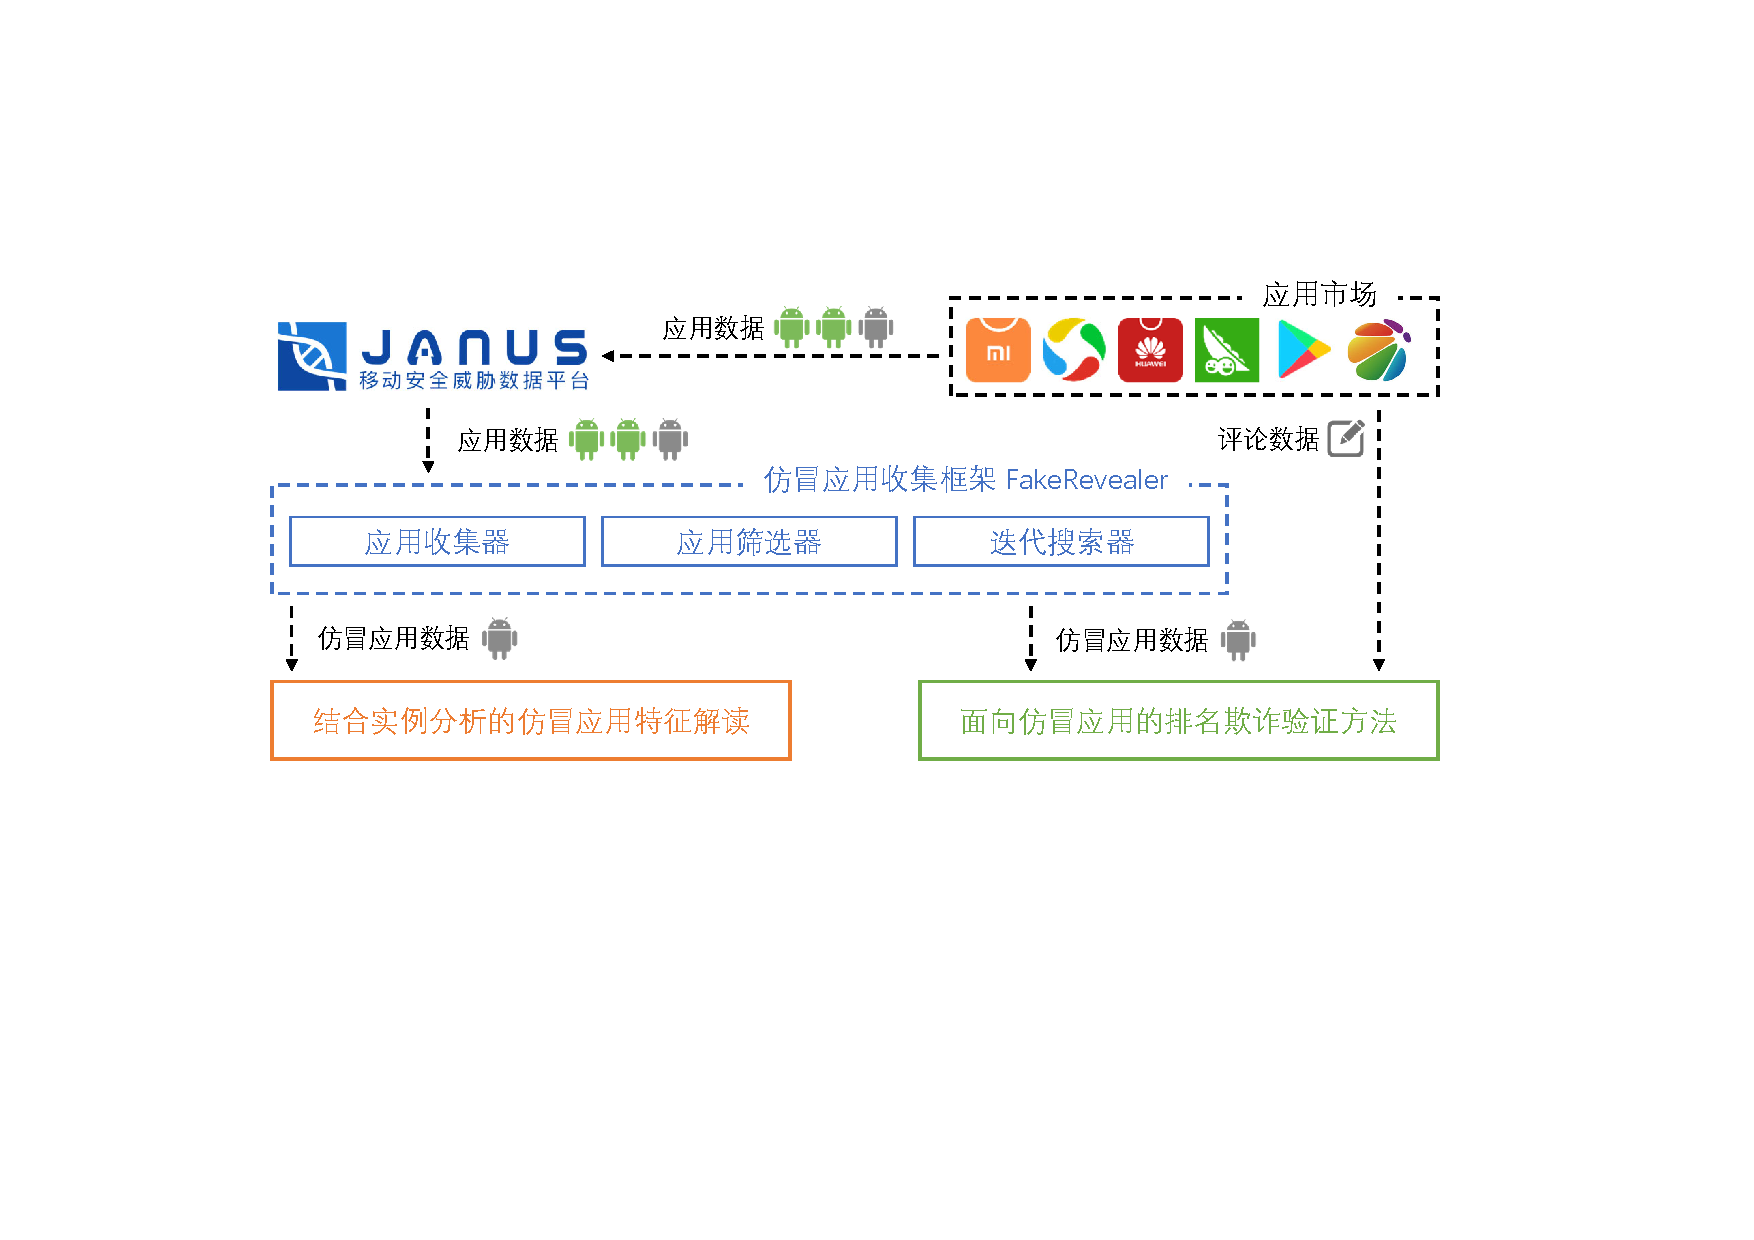
\includegraphics[width=\textwidth]{./Figures/edwin-overview}
% 	\caption{本文工作概览}
% 	\label{fig:Workflow}
% 	\vspace{-3mm}
% \end{figure}
%
% 本节为本文工作提供概览。如\autoref{fig:Workflow}所示,本工作通过三个主要部分,完成三部分工作:
%
% 1)\ \emph{利用面向仿冒应用的收集框架\mytool 收集大规模数据,解决仿冒应用数据稀缺的问题} \quad
% 针对实证研究中实验数据应尽可能具有完整性与代表性的要求,本研究设计并实现了仿冒应用收集框架\mytool,尽可能全面地进行仿冒应用的数据收集。
% 数据收集主要分为两个部分:正版应用信息的收集和仿冒应用的收集。
% 在正版应用信息收集的部分,本文选择了50个最热门的App作为目标应用,然后手动收集了跟这些App有关的信息;
% 基于该50款目标应用,本研究利用\mytool,收集了从29个应用来源获得的近14万个应用样本,并从中筛选出5万个仿冒应用,整理成集。
% 该数据集可为后续相关工作如代码分析、特征检测等提供数据支持。
%
% 2)\ \emph{首次针对仿冒应用的特性进行大规模的特征解读} \quad
% 针对移动黑灰产研究中关于仿冒应用的研究空白,本研究利用上述仿冒应用数据,结合案例分析,进行了首次基于Android系统仿冒应用的大规模特征解读。
% 特征解读从三个视角完成,这些视角分别是仿冒的基本应用特征、影响仿冒应用数量的因素和仿冒应用的发展轨迹,由浅入深揭示仿冒应用的生态。
% 对应的三个案例分析除了为特征解读提供案例支持之外,还揭示了更多仿冒应用开发者的行为特征,可为用户、应用市场和安全领域从业人员等多方受众提供一定见解。
%
% 3)\ \emph{面向仿冒应用的排名欺诈验证} \quad
% 该部分中,本文从第三方应用市场中随机选取一部分应用,爬取用户对它们的所有历史评价,以检测仿冒应用与排名欺诈行为的关联。
% 针对前人检测研究需要先验知识或特殊数据的问题,本研究从社交媒体研究引入了用户行为可信度进行排查,避开了现有方法的局限性。
% 进一步地,本研究从评论内容重复率方面提出了另一创新性排查方法,解决了数据量增大带来的大运算量问题。
% 人工复查结果显示,两种排查方法均取得了优于现有方法的结果。
\section{本文组织结构}
% todo: 7 chapters?
本文共分为七章,环绕着本研究的数据搜集和不同的分析方向展开,各章节内容如下:

\fullref{chp:intro} 主要提供了本文的研究背景、相关工作、本文采用的研究方法、关键问题分析与本文的主要工作。

\fullref{chp:background} 介绍相关技术背景,从软件工程领域的实证研究出发,介绍实证研究的常用方法和数据收集、验证标准等理论背景,再着眼于本研究的主体——Android应用,介绍了Android安全证书机制和与仿冒应用相关的重打包技术。

\fullref{chp:research_settings} 介绍整个研究的设置,包括根据研究现状提出研究问题、确立研究对象,阐述数据收集的相关考量,并与其他研究收集的数据进行对比。

\fullref{chp:discoveries_basic} 从仿冒应用与原版应用相似度、影响应用被仿冒的严重程度的因素及仿冒应用行为三点入手,对与仿冒应用基本特征相关的三个方面进行实证研究,最后针对研究结果分别向用户、应用市场和应用开发者提供实用建议。

\fullref{chp:discoveries_behavior} 则结合应用证书视角与结合时间维度视角进行探索,分析现有应用市场监管策略存在的不足,针对性地提出改善措施。

以前两章实证研究所得的经验作参考,作者于\fullref{chp:framework_prototype} 提出并实现了一个仿冒应用检测框架,并基于新采集的应用数据对框架进行了有效性检验。

% % 这些视角包括仿冒应用特征、影响仿冒应用数量的因素和仿冒应用的发展轨迹,每个视角都被进一步分解成多个不同的研究问题。
% % 说明仿冒应用的数据收集方式并详细介绍其中三个组件(\componentA、\componentB 和\componentC)的设计与实现,
% % 结束解读后,本文从数据中挑选三个具有代表性的案例进行分析,以案例进一步深化分析结果。

% \fullref{chp:feedback} 针对仿冒应用进行了排名欺诈检测。
% 针对现有检测方法的不足,本文先后提出两个具有创新性的方法对排名欺诈行为进行排查,并将排查结果与前一章的仿冒应用进行比对。
% % 结果显示,仿冒应用存在排名欺诈行为。仿冒应用与排名欺诈行为作为移动黑灰产的两个环节存在关联。

\fullref{chp:future} 对本文工作进行总结,并对下一步工作进行展望。
